\documentclass[11pt]{article}

%\usepackage{filecontents}

\usepackage{pgfplots}
\usepgfplotslibrary{groupplots}
%\pgfplotsset{compat=1.14}

\usepackage{xcolor}

\definecolor{riptide}{RGB}{141,211,199}
\definecolor{pale_prim}{RGB}{255,255,179}
\definecolor{lavender_gray}{RGB}{190,186,218}
\definecolor{salmon}{RGB}{242,131,107}
\definecolor{seagull}{RGB}{128,177,211}
\definecolor{rajah}{RGB}{253,180,98}
\definecolor{yellow_green}{RGB}{198,222,119}
\definecolor{classic_rose}{RGB}{252,205,229}
\definecolor{feijoa}{RGB}{178,223,138}

\definecolor{cruise}{RGB}{179,226,205}
\definecolor{apricot}{RGB}{253,205,172}
\definecolor{periwinkle}{RGB}{203,213,232}
\definecolor{snow_flurry}{RGB}{230,245,201}
\definecolor{buttermilk}{RGB}{255,242,174}

\definecolor{sundown}{RGB}{249, 180, 181}
\definecolor{spindle}{RGB}{179,205,227}
\definecolor{tea_green}{RGB}{204,235,197}
\definecolor{languid_lavender}{RGB}{222,203,228}
\definecolor{champagne}{RGB}{254,217,166}
\definecolor{cream}{RGB}{255,255,204}


\definecolor{nonte_carlo}{RGB}{135,204,194}
\definecolor{melon}{RGB}{254,191,181}
\definecolor{granny_smith_apple}{RGB}{150,214,150}
\definecolor{mona_lisa}{RGB}{246,152,134}
\definecolor{watusi}{RGB}{254,221,207}
\definecolor{see_green}{RGB}{161,228,195}

\definecolor{moss_green}{RGB}{170,216,176}
\definecolor{opal}{RGB}{164,207,190}

\definecolor{pale_turquoise}{RGB}{172,240,242}
\definecolor{Madang}{RGB}{190,235,159}
\definecolor{pixie_green}{RGB}{183,214,170}
\definecolor{coral_andy}{RGB}{243,204,205}
\definecolor{manhattan}{RGB}{226,180,125}
\definecolor{quartz}{RGB}{219,223,238}
\definecolor{spring_sun}{RGB}{242,243,195}
\definecolor{dairy_cream}{RGB}{254,226,189}
\definecolor{surf_crest}{RGB}{205,230,208}
\definecolor{french_pass}{RGB}{195,232,246}
\definecolor{cosmos}{RGB}{248,209,210}
\definecolor{portafino}{RGB}{245,237,160}
\definecolor{sail}{RGB}{163,205,235}
\definecolor{hint_green}{RGB}{226,246,209}


\definecolor{jet_stream}{RGB}{188, 214, 210}


\definecolor{azalea}{RGB}{251, 196, 196}
\definecolor{wewak}{RGB}{244, 143, 150}
\definecolor{bittersweet}{RGB}{255,111,105}
\definecolor{sunset_orange}{RGB}{242,89,75}
\definecolor{light_coral}{RGB}{244, 127, 123}
\definecolor{carnation}{RGB}{245, 80, 86}
\definecolor{flamingo}{RGB}{237, 88, 85}
\definecolor{carmine_pink}{RGB}{231, 76, 60}
\definecolor{deep_carmine_pink}{RGB}{236, 50, 67}
\definecolor{fire_engine_red}{RGB}{210,44,41}
\definecolor{amaranth}{RGB}{234,46,73}
\definecolor{ku_crimson}{RGB}{243, 0, 25}
\definecolor{fire_engine_red}{RGB}{206, 37, 51}
\definecolor{copper_rust}{RGB}{155, 64, 74}

\definecolor{chilean_fire}{RGB}{215, 87, 44}

\definecolor{japanese_laurel}{RGB}{53, 116, 40}


\definecolor{turmeric}{RGB}{211, 178, 76}
\definecolor{saffron}{RGB}{249,193,62}
\definecolor{my_sin}{RGB}{255, 176, 59}
\definecolor{tree_poppy}{RGB}{246, 154, 27}
\definecolor{jaffa}{RGB}{240, 131, 58}
\definecolor{crusta}{RGB}{254, 127, 44}
\definecolor{tahiti_gold}{RGB}{223, 102, 36}
\definecolor{outrageous_orange}{RGB}{255, 100, 45}
\definecolor{safety_orange}{RGB}{254, 106, 0}



\definecolor{turquoise}{RGB}{41,217,194}
\definecolor{puerto_rico}{RGB}{94, 194, 166}
\definecolor{mountain_meadow}{RGB}{0, 163, 136}
\definecolor{free_speech_aquamarine}{RGB}{0, 156, 114}
\definecolor{java}{RGB}{2,190,196}


% person:
\definecolor{matisse}{RGB}{25, 104, 167}
\definecolor{shakespeare}{RGB}{85, 154, 193}
\definecolor{mona_lisa}{RGB}{246,152,134}

% gray:
\definecolor{bgc}{RGB}{245,245,245}
\definecolor{tuatara}{RGB}{67, 67, 67}
\definecolor{aluminum}{RGB}{153,153,153}
\definecolor{silver}{RGB}{191,191,191}
\definecolor{platinum}{RGB}{228,228,228}
\definecolor{mercury}{RGB}{230,230,230}
\definecolor{gallery}{RGB}{240,240,240}
\definecolor{athens_gray}{RGB}{236, 240, 241}

% nature color
\definecolor{early_dawn}{RGB}{252,243,218}
\definecolor{egg_shell}{RGB}{238, 234, 215}
\definecolor{midnight}{RGB}{0, 29, 50}
\definecolor{sundown}{RGB}{249, 180, 181}
\definecolor{sun_shade}{RGB}{255, 144, 68}
\definecolor{sushi}{RGB}{117, 168, 47}
\definecolor{tomato}{RGB}{255, 97, 56}
\definecolor{ice_cold}{RGB}{169,232,220}


% blue:
\definecolor{jelly_bean}{RGB}{45, 126, 150}
\definecolor{shakespeare}{RGB}{85, 154, 193}
\definecolor{celestial_blue}{RGB}{52, 152, 219}
\definecolor{curious_blue}{RGB}{41, 128, 185}
\definecolor{french_blue}{RGB}{0, 112, 182}
\definecolor{matisse}{RGB}{25, 104, 167}

\definecolor{biscay}{RGB}{44, 62, 80}

% green:
\definecolor{cosmic_latte}{RGB}{222, 247, 229}
\definecolor{chinook}{RGB}{163, 232, 178}
\definecolor{padua}{RGB}{121, 189, 143}
\definecolor{ocean_green}{RGB}{79, 176, 112}
\definecolor{pastel_green}{RGB}{107, 227, 135}
\definecolor{chateau_green}{RGB}{69, 191, 85}
\definecolor{RoyalBlue}{RGB}{69, 191, 85}
\definecolor{pigment_green}{RGB}{0, 175, 79}
\definecolor{fern}{RGB}{101,197,117}
\definecolor{killarney}{RGB}{56, 113, 66}
\definecolor{viridian}{RGB}{70, 137, 102}


\definecolor{jet_stream}{rgb}{0.69,0.61,0.85}
\definecolor{jelly_bean}{rgb}{0.47,0.32,0.66}




%\begin{filecontents*}{cl}
%-0.5, 2
%-0.45, 2
%-0.4, 2
%-0.35, 2
%-0.3, 5
%-0.25, 2
%-0.2, 10
%-0.15, 20
%-0.1, 11
%-0.05, 13
%0.0, 20
%0.05, 15
%0.1, 27
%0.15, 28
%0.2, 30
%0.25, 40
%0.3, 70
%0.35, 74
%0.4, 79
%0.45, 103
%0.5, 111
%0.55, 151
%0.6, 157
%0.65, 191
%0.7, 182
%0.75, 200
%0.8, 207
%0.85, 166
%0.9, 114
%0.95, 26
%\end{filecontents*}
%
%\begin{filecontents*}{sas}
%-0.35, 1
%-0.3, 6
%-0.25, 3
%-0.2, 12
%-0.15, 9
%-0.1, 19
%-0.05, 33
%0.0, 26
%0.05, 34
%0.1, 37
%0.15, 45
%0.2, 37
%0.25, 57
%0.3, 75
%0.35, 107
%0.4, 147
%0.45, 157
%0.5, 186
%0.55, 212
%0.6, 211
%0.65, 170
%0.7, 177
%0.75, 144
%0.8, 98
%0.85, 39
%0.9, 7
%0.95, 11
%\end{filecontents*}

\begin{document}


\begin{figure}
\pgfplotsset{
axis background/.style={fill=gallery},
grid=both,
  xtick pos=left,
  ytick pos=left,
  tick style={
    major grid style={style=white,line width=.5pt},
    minor grid style={style=white, line width=.1pt},
    draw=none
    },
  ytick={200, 400},
  every x tick label/.append style={font=\tiny, yshift=2pt},
  every y tick label/.append style={rotate=90, font=\fontsize{1pt}{1pt}\selectfont, yshift=-2pt},
  ymajorgrids,
	major grid style={draw=white},
	y axis line style={opacity=0},
	tickwidth=0pt,
  title style={yshift=-5ex, font=\small},
  y label style={yshift=-5pt},
  minor tick num=1,
  height=0.4\linewidth,
  width=0.9\linewidth,
  ymin=0, ymax=600
}
\centering
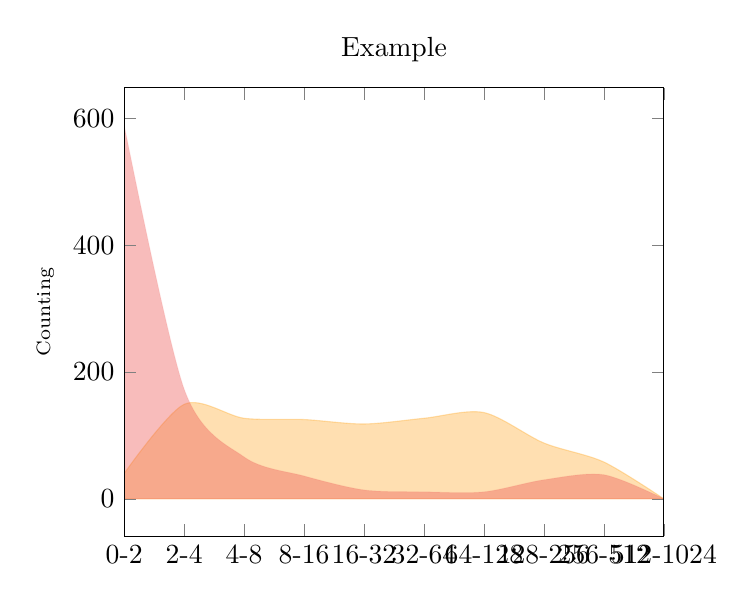
\begin{tikzpicture}
	\begin{axis}[
		smooth,
		%stack plots=y,
		area style,
		enlarge x limits=false,
		xticklabels={0-2, 2-4, 4-8, 8-16, 16-32, 32-64, 64-128, 128-256, 256-512, 512-1024},
	    xtick={1,2,3,4,5,6,7,8,9,10},
	    ylabel={\scriptsize Counting},
	    title={Example},
	    ]
	\addplot[color=my_sin, fill=my_sin, opacity=0.4] coordinates
		{(1, 40) (2, 149) (3, 127) (4, 125) (5, 118) (6, 127) (7, 136) (8, 88) (9, 58) (10, 0)}
		\closedcycle;
	
	\addplot[color=flamingo, fill=flamingo, fill opacity=0.4, draw opacity=0.1] coordinates
		{(1,589) (2,173) (3,66) (4,36) (5,14) (6,11) (7,11) (8,30) (9,38) (10,0)}
		\closedcycle;
	\end{axis}
\end{tikzpicture}

  \caption{Dist plot.}
  \label{rank_distribution}
\end{figure}




\begin{figure}
\pgfplotsset{
axis background/.style={fill=gallery},
grid=both,
  xtick pos=left,
  ytick pos=left,
  tick style={
    major grid style={style=white, line width=1pt},
    minor grid style=white,
    draw=none,
  },
  minor tick num=1,
}
\centering
\resizebox{0.8\textwidth}{!}{
    \begin{tikzpicture}
      \begin{axis}[
        %axis on top,
        % enlarge x limits=0.05,
        xlabel=\huge Example,
        ylabel=\huge Count,
        ymin=0, ymax=220, ytick distance=20,
        xmax=1, xmin=-1, xtick distance=0.1,
        % minor xtick={-0.95, -0.85, ..., 0.95},
        % xtick={-1, -0.9, ..., 1},
        x tick label style={
        % yshift=-3mm,
        % rotate=-90, 
        % anchor=base, 
        font=\normalsize,
        scaled ticks=false,
        /pgf/number format/fixed,
        /pgf/number format/precision=2},
        y tick label style={
        font=\Large,
        },
        % extra x ticks={1},
        y label style={
         yshift=3mm
        },
        x label style={
         yshift=-2mm
        },
        legend style={
          % nodes={scale=2, transform shape},
          legend image post style={scale=3},
          font=\Large,
          fill=gallery,
          draw=none,
          draw opacity=0,
          legend cell align=left,
          legend columns=1,
          at={(0.1, 0.97)},
          anchor=north,
          row sep=2mm,
          column sep=2mm,
          /tikz/every even column/.append style={column sep=1mm}
        },
        width=2\textwidth,
        ybar=0pt, %  configures ‘bar shift’
        bar shift=0pt,
        bar width=15pt,
        ymajorgrids,
        major grid style={draw=white},
        y axis line style={opacity=0},
        tickwidth=0pt,
        % nodes near coords,
        legend entries = {cl, sas}
        ]
        \addplot[draw=none, fill=summer_sky, opacity=0.5] coordinates {
        (-0.9, 0)
        (-0.50, 2)
        (-0.45, 2)
        (-0.40, 2)
        (-0.35, 2)
        (-0.30, 5)
        (-0.25, 2)
        (-0.20, 10)
        (-0.15, 20)
        (-0.10, 11)
        (-0.05, 13)
        (0.00, 20)
        (0.05, 15)
        (0.10, 27)
        (0.15, 28)
        (0.20, 30)
        (0.25, 40)
        (0.30, 70)
        (0.35, 74)
        (0.40, 79)
        (0.45, 103)
        (0.50, 111)
        (0.55, 151)
        (0.60, 157)
        (0.65, 191)
        (0.70, 182)
        (0.75, 200)
        (0.80, 207)
        (0.85, 166)
        (0.90, 114)
        (0.95, 26)
          };        
        \addplot[draw=none, fill=flamingo, opacity=0.5] coordinates {
        (-0.35, 1)
        (-0.30, 6)
        (-0.25, 3)
        (-0.20, 12)
        (-0.15, 9)
        (-0.10, 19)
        (-0.05, 33)
        (0.00, 26)
        (0.05, 34)
        (0.10, 37)
        (0.15, 45)
        (0.20, 37)
        (0.25, 57)
        (0.30, 75)
        (0.35, 107)
        (0.40, 147)
        (0.45, 157)
        (0.50, 186)
        (0.55, 212)
        (0.60, 211)
        (0.65, 170)
        (0.70, 177)
        (0.75, 144)
        (0.80, 98)
        (0.85, 39)
        (0.90, 7)
        (0.95, 11)
          }; 
      \end{axis}
    \end{tikzpicture}}
    
\end{figure}



\end{document}
